\documentclass[11pt,a4paper]{article}
\ifdefined\pdfminorversion\pdfminorversion=7\fi
\usepackage[T1]{fontenc}
\usepackage[utf8]{inputenc}
\usepackage{lmodern}
\usepackage[a4paper,margin=25mm,headheight=14pt]{geometry}
\usepackage{amsmath,amssymb}
\usepackage{booktabs}
\usepackage{enumitem}
\usepackage{microtype}
\usepackage{tabularx}
\usepackage{xcolor}
\usepackage{pid-rs-report-tables}
\usepackage{float}
\usepackage[unicode]{hyperref}
\usepackage{xurl}
\usepackage{fancyhdr}
\usepackage{graphicx}

\newcolumntype{L}[1]{>{\raggedright\arraybackslash}p{#1}}
\newcolumntype{Y}{>{\raggedright\arraybackslash}X}
\setlength{\emergencystretch}{3em}

\ifdefined\pdfinfoomitdate\pdfinfoomitdate=1\fi
\ifdefined\pdftrailerid\pdftrailerid{}\fi
\ifdefined\pdfsuppressptexinfo\pdfsuppressptexinfo=15\fi
\hypersetup{%
  hidelinks,
  pdftitle={KSG revision-4 M1a composite-v7 dual-defect boundary},
  pdfauthor={Sepehr Mahmoudian},
  pdfsubject={Append-only correction of two distinct C6 operational defects},
  pdfkeywords={KSG, evidence custody, local closure, hosted qualification, append-only repair}
}

\newcommand{\Important}[1]{\textcolor{PidPrimary}{\textbf{#1}}}

\PidConfigureSections
\PidSetRunningHeads{pid-rs composite-v7}{KSG dual-defect operational boundary}
\PidConfigureAbstract
\PidConfigureLinksAndListings

\setlength{\parindent}{0pt}
\setlength{\parskip}{5pt}
\setlist{nosep,leftmargin=5mm}
\renewcommand{\arraystretch}{1.17}

\title{\PidReportTitle
  {KSG Revision-4 M1a Composite-v7 Operational Boundary}
  {Two distinct C6 defects; one append-only successor}}
\author{pid-rs project analysis}
\date{18 August 2026}

\begin{document}
\PidMakeTitle

\begin{abstract}
Published C6 commit
\path{0c3afa0ab5b264370072a18d24655df35b90574c} has two distinct operational
defects. First, its immutable local recorder requires exact authority blobs larger than the
65,536-byte cap applied to every internal command, so no honest L6 record can satisfy its own
contract. Second, its dedicated and repository-CI attempt-1 lanes reached the same
\texttt{missing command: rg} marker because \texttt{ripgrep} was omitted from their package
declarations. Those hosted manifestations are correlated observations of one dependency defect,
not independent evidence, and they do not evidence PDF-content failure. R6 is permanently
unissued. Direct-child C7 preserves every v6 publication and gate byte, adds a 2 MiB channel only
for exact authority reads while retaining 64 KiB for generic probes, and closes the exact
\texttt{ripgrep}-package/\texttt{rg}-probe dependency. R7 remains conditional on fresh exact-C7
local and attempt-1 hosted success. No theorem, estimator, PID object, or numerical result changes.
\end{abstract}

\begin{center}
\fcolorbox{PidAccent}{PidSoft}{\parbox{0.92\linewidth}{%
\Important{Disposition.} C6 remains the immutable published subject. R6 is permanently absent.
C7 is an append-only direct child that repairs two bounded operational contracts; it does not
reinterpret C6 or transfer qualification credit. R7 may exist only after all four fresh C7 terms
are true. This record grants no science, mathematics, security, application, authentication,
authorship, trusted-time, hermeticity, independence, PDF/UA, or renderer-independence credit.
}}
\end{center}

For exact C6 define
\begin{equation}
  Q_6=L_6\land\mathrm{CI}_6\land\mathrm{CodeQL}_6\land D_6,
  \label{eq:q6}
\end{equation}
where L6 is an unnumbered local observation and the three hosted terms require terminal success at
attempt 1 for the same commit. Both the impossible local contract and hosted failure make the
conjunction false. The immutable issuance rule
\begin{equation}
  \operatorname{issue}(R6)\Longleftrightarrow Q_6
  \label{eq:r6}
\end{equation}
therefore leaves R6 permanently unissued. It may not be reconstructed, renamed, backdated, or
inferred from later evidence.

\clearpage
\section{Defect one: the local authority-stream contradiction}

The exact C6 recorder sorts this required authority inventory by path:

\begin{table}[H]
\centering
\small
\begin{tabularx}{\linewidth}{@{}Y L{0.12\linewidth} L{0.20\linewidth}@{}}
\toprule
\PidTableHeaderRow
\textbf{Authority path} & \textbf{Bytes} & \textbf{Relation to 65,536} \\
\midrule
local-closure schema v6 & 13,620 & below \\
\texttt{justfile} & 32,358 & below \\
local recorder v6 & 57,021 & below \\
composite-v6 self-test & 69,573 & above; first failure \\
composite-v6 checker & 124,520 & above \\
\bottomrule
\end{tabularx}
\caption{The final two required committed blobs exceed the immutable internal-command stream cap.}
\label{tab:authority-sizes}
\end{table}

The exact source route is
\begin{center}
\small
\texttt{authority\_descriptors} $\longrightarrow$ \texttt{git\_output}
$\longrightarrow$ \texttt{internal\_command} $\longrightarrow$ \texttt{run\_bounded}.
\end{center}
The internal-command wrapper supplies \(64\times1024=65{,}536\) bytes for every caller, yet the
authority contract requires the full returned bytes to equal the stable mode-0644 worktree file.
Exact equality and acceptance of either oversized committed blob cannot both hold.

The canonical closed counterexample is
\path{audit/evidence/ksg-rev4-m1a-composite-v6-local-closure-counterexample-v7-2026-08-18.json},
SHA-256
\path{cabcd565f25e11d14c4082532ea7efe1987eb0d700c115a8fbf36937486eede2}, 9,103 bytes.
Its schema is
\path{audit/schemas/ksg-rev4-m1a-composite-local-closure-counterexample-v7.schema.json}, SHA-256
\path{d06f0437cd5eddce35a88be9eccd5653ddc36b29b361ff924c33578d15a4de7b}, 21,621 bytes.
The checker exact-binds the full Draft 2020-12 schema bytes, dialect, identifier, and closed root,
then rederives the evidence semantics directly without schema stripping or a claim that the
repository subset evaluator implements every full-Draft keyword.
The artifact binds source, blob identity, size, and the contradiction. It does not invent a more
specific runtime trace, authenticate the repository, or establish the absence of other defects.

\section{C7 local repair predicate}

C7 retains the immutable v6 65,536-byte per-stream wrapper for version, configuration, status, and
other inherited generic probes. A new v7 committed-authority wrapper alone explicitly selects the
2,097,152-byte bound already applied to worktree authority files. It reads the hardcoded authority
path from the validated exact C7 commit, not from a floating literal \texttt{HEAD}. The returned
committed bytes must still equal the stable mode-0644 worktree bytes.

The boundary suite accepts 65,536 bytes and rejects 65,537 bytes in the generic lane; it accepts
65,537 and 2,097,152 bytes and rejects 2,097,153 bytes in the authority lane. It also rejects
truncation, mutation, nonzero exit, stderr, timeout, wrong path or object, symlink, hardlink, wrong
mode, drift, and any mutation that globally widens the 64 KiB generic limit.

The fixed local command is \texttt{just ksg-composite-v7}. A valid L7 record binds that command,
one exact clean C7 pre/post observation, bounded output, a minimal environment, and the reviewed
executable roster. This remains correlated unsigned operational evidence, not authentication,
trusted time, complete executable inventory, or hermetic execution.

\clearpage
\section{Defect two: one hosted dependency declaration}

The exact hosted marker is
\begin{center}
\texttt{composite publication PDF v6 adjudication: missing command: rg}.
\end{center}
It identifies a command-availability precondition failure. It is not evidence that any report,
figure, receipt, TeX source, or PDF-content predicate failed.

\begin{table}[H]
\centering
\small
\begin{tabularx}{\linewidth}{@{}L{0.22\linewidth}L{0.25\linewidth}Y@{}}
\toprule
\PidTableHeaderRow
\textbf{Route} & \textbf{Run / state} & \textbf{Bounded observation} \\
\midrule
Dedicated v6 & \texttt{32139920743}; failed & Attempt 1 had sole failure job \texttt{95719898016}; its step 9 exited 2 at the exact missing-\texttt{rg} marker. \\
Repository CI & \texttt{32139920717}; failed & Attempt 1 completed with 45 terminal jobs: 44 success and sole failure job \texttt{95719898423}; no other non-success. Its step 11 exited 2 at the same marker. \\
CodeQL & \texttt{32139921184}; passed & Attempt 1 jobs \texttt{95719905024}, \texttt{95719905101}, \texttt{95719905184}, and \texttt{95719905296} succeeded; this term cannot transfer across the false C6 conjunction. \\
\bottomrule
\end{tabularx}
\caption{Terminal exact-C6 hosted observations. The repository-CI roster completed at
14:48:10Z on 18 August 2026.}
\label{tab:c6-hosted}
\end{table}

The sole failed CI job is \emph{Formal LaTeX / PDF inventory and cross-toolchain structure}; its
step 11 is \emph{Rebuild papers and check cross-toolchain text, geometry, fonts, and workflow
renders}.

The installed predecessor capture is
\path{audit/evidence/ksg-rev4-m1a-composite-predecessor-failure-hosted-capture-v7-2026-08-18.json},
mode 0644 and 1,819,338 bytes, with raw SHA-256
{\small\mbox{\texttt{e9a1d574cb4127263d8aaec3e291e78836b849f9b402af8a0daa5eb37cc70104}}};
its normalized role digest is
{\small\mbox{\texttt{bc81849000b3967b9f3a226629e39cfe754fc2cf951294a94fc319a41ac0f9e8}}}.
It binds 36 retained response rows across two retrieval repetitions, zero retry events, and 1,349,170
retained body bytes.

The stable raw job-log bindings are SHA-256
\path{b1665fe7c8573a1df1e47ea78cbe39c804a960ec1f8aabcc79c23be574ec0960} for the
dedicated job and
\path{166e1d703f81c080adecc7a6bc3f366bf66b11708b3c31b3ea1cd121fcd94460} for the
repository-CI failed job. These are content bindings, not provider authentication.

The dedicated and CI manifestations share the same omitted package declaration and diagnostic
surface. They are correlated observations of one missing-\texttt{ripgrep} defect, not two defect
classes and not independent evidence. C7 adds the named \texttt{ripgrep} apt package to the
repository-CI formal-PDF block and dedicated-v7 installation list. Each hosted lane requires
\texttt{command -v rg} to resolve exactly to \texttt{/usr/bin/rg} and executes
\texttt{/usr/bin/rg --version}; the apt package itself is not byte-pinned. The local recorder
separately resolves and binds \texttt{rg} in its reviewed executable roster. This closes the named
package/probe contract; it is not a claim of complete dependency closure, provider authenticity,
or hermetic execution.

Every v6 PDF, TeX source, SVG, rendering receipt, visual receipt, comparator, publication gate,
and hostile suite stays byte-exact. The C7 publication is a new versioned lane. It may not revise
the C6 failure evidence to claim a PDF-content defect that the logs never reached.

\clearpage
\section{Append-only C6 to C7 topology}

C7 must be the exact unsigned single-parent direct child of C6. There is no R6 commit between them.
Replay r11 is the finalized C6-era predecessor replay; fresh r12 is the current C7 replay cut.
Define
\begin{equation}
  Q_7=L_7\land\mathrm{CI}_7\land\mathrm{CodeQL}_7\land D_7,
  \label{eq:q7}
\end{equation}
where L7 is one unnumbered local observation for exact C7. The three hosted terms require fresh
terminal attempt-1 success for that same commit. The issuance policy is
\begin{equation}
  \operatorname{issue}(R7)\Longleftrightarrow Q_7.
  \label{eq:r7}
\end{equation}
Any false, absent, nonterminal, retry, wrong-commit, or wrong-attempt hosted term leaves R7
unissued and requires another append-only successor.

\begin{figure}[H]
\centering
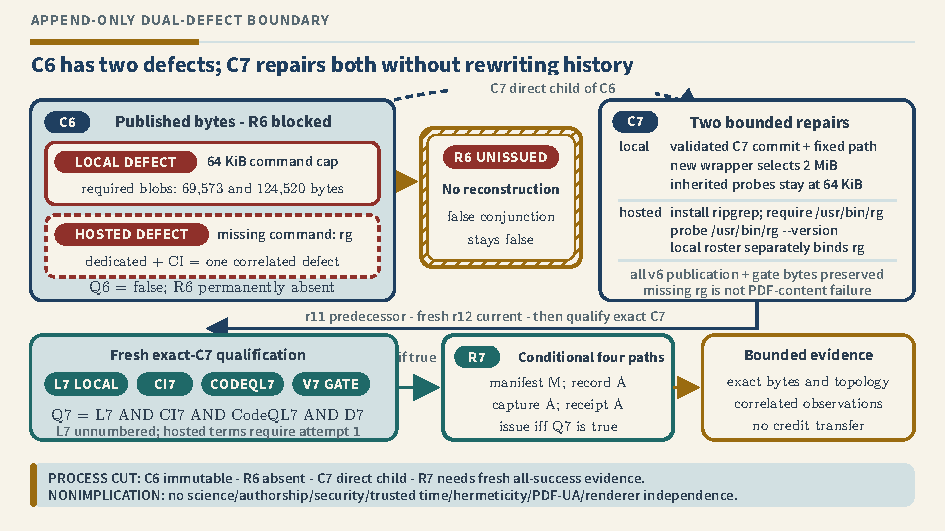
\includegraphics[
  width=\linewidth,
  alt={Published C6 has two distinct operational defects. Its local recorder applies a 65,536-byte
  internal-command cap to required 69,573-byte and 124,520-byte authority blobs. Its dedicated and
  repository-CI attempt-1 lanes also reach one correlated missing-rg dependency-declaration
  failure, which is not PDF-content failure. R6 remains permanently unissued. Direct-child C7 adds
  an authority-only 2 MiB path while retaining generic 64 KiB bounds, installs ripgrep, resolves rg,
  and preserves every v6 publication and gate byte. Only unnumbered L7 plus fresh attempt-1 CI7,
  CodeQL7, and dedicated-v7 success can permit an exact four-path R7.}
]{figures/ksg-m1a-composite-v7-boundary/c6-failure-c7-r7.pdf}
\caption{Append-only dual-defect boundary. Shape, line style, text, and color separately distinguish
the local contradiction, hosted dependency defect, absent R6, bounded C7 repairs, and conditional
R7 route.}
\label{fig:v7-boundary}
\end{figure}

If and only if \(Q_7\) is true, R7 is the exact direct child of C7 and has exactly these four path
changes:
\begin{itemize}
  \item modify \path{audit/evidence/current-source-state-v1.json};
  \item add \path{audit/evidence/ksg-rev4-m1a-composite-local-closure-v7-2026-08-18.json};
  \item add \path{audit/evidence/ksg-rev4-m1a-composite-successor-qualification-hosted-capture-v7-2026-08-18.json}; and
  \item add \path{audit/evidence/ksg-rev4-m1a-composite-receipt-v7-2026-08-18.json}.
\end{itemize}
The receipt derives all four terms only after validating the durable local record and fresh hosted
capture; the self-excluding current-source manifest is regenerated last.

\clearpage
\section{Publication gate and causal controls}

The v7 publication set contains an ARIA-labelled SVG with title and description, a TeX text
alternative, deterministic standalone figure PDF, five-page report PDF, 120-dpi rendering receipt,
and 144-dpi visual-review receipt. The gate checks exact byte bindings and two isolated
same-toolchain rebuilds before applying cross-toolchain structure and raster bounds.

\begin{table}[H]
\centering
\small
\begin{tabularx}{\linewidth}{@{}L{0.23\linewidth}Y@{}}
\toprule
\PidTableHeaderRow
\textbf{Surface} & \textbf{Fail-closed predicate and causal control} \\
\midrule
Sources & Exact boundary, counterexample, schema, TeX, SVG, PDFs, receipts, and comparator bind; omission or mutation rejects. \\
Claims & Two defects remain distinct; hosted duplicates stay correlated; missing \texttt{rg} cannot become PDF-content failure; bound and topology drift reject. \\
Object safety & Unsupported catalog, outline, or page actions; annotations; embedded files; missing resources; nonidentity matrices; inline images; and raster images reachable through Forms, patterns, Type~3 fonts, or soft masks reject. \\
Placement & Clipping, wrong page, off-page placement, zero scale, rotation, altered page boxes, and altered user units reject. \\
Text and fonts & Closed headings/body order, embedded subset fonts, encodings, widths, Unicode maps, programs, and report/figure font inventories are checked. \\
Raster & Color and grayscale comparisons use one local Poppler with explicit bounds; a visible overlay rejects. \\
Receipt & Exact render rows, hashes, sizes, review pages, figure placements, and ordered prose are closed; drift or extra claims reject. \\
\bottomrule
\end{tabularx}
\caption{Hostiles reseal outer byte bindings so rejection must reach the named predicate.
Checksum-only rejection receives no causal-test credit.}
\label{tab:controls}
\end{table}

Same-renderer comparison is correlated differential evidence. It is not renderer independence,
PDF/UA conformance, absolute visual correctness, or a general portability theorem. The clean
endpoints use ordinary Git status plus selected metadata checks; repository-ignored products and
uninspected Git metadata remain outside the observation and may remain side inputs, so this is not
a hermetic closure.

\section{Scope boundary}

Composite-v7 adds zero PID theories, zero PID functionals, zero estimators, zero theorem-source
changes, and zero numerical-result changes. Nothing transfers among categorical or continuous
shared exclusions, KSG mutual information, Williams--Beer \(I_{\min}\), PID2, PID3, quantized, or
mixed-support routes.

Hash equality binds named bytes only. This report establishes no authentication, attestation,
authorship, provider completeness, trusted time, peer review, dependency-disjoint independence,
scientific or mathematical validity, security certification, privacy assurance, application
fitness, safety, control authority, archival preservation, PDF/UA accessibility, or renderer
independence.

\end{document}
